\chapter*{Appendix A: Exploratory Data Analysis of the NYC Yellow Taxi Dataset}
\addcontentsline{toc}{chapter}{Appendix A: Exploratory Data Analysis}

\textit{This appendix provides a detailed exploratory analysis of the NYC Yellow Taxi dataset, including schema validation, business rule checks, and data quality observations. These findings motivate the CA-DQStream framework design presented in Chapter 3.}

% ================================================
% A.1 Case Study: NYC Yellow Taxi Dataset
% ================================================
\section{Case Study: NYC Yellow Taxi Dataset}

We use the NYC Yellow Taxi dataset as our case study. The dataset is published by the NYC Taxi and Limousine Commission (TLC) and contains trip records for all yellow medallion taxis. We analyze 3,076,903 records from July 2024, with temporal validation across 26 months (January 2024 -- February 2026).

\subsection{Dataset Schema}

The dataset contains 19 raw columns plus 4 derived features computed during preprocessing. Key columns include:

\begin{itemize}
    \item \textbf{VendorID:} Integer identifier for the TPEP provider (1=CMT, 2=VTS, 6=Unknown).
    \item \textbf{tpep\_pickup\_datetime / tpep\_dropoff\_datetime:} Pickup and dropoff timestamps.
    \item \textbf{passenger\_count:} Number of passengers (NULL indicates a completeness violation).
    \item \textbf{trip\_distance:} Trip distance in miles (must be $> 0$).
    \item \textbf{RatecodeID:} Rate category (1=Standard, 2=JFK, 3=Newark, 4=Negotiated, 5=Group, 6=Shared, 99=Unknown). This is the key context dimension for CA-DQStream.
    \item \textbf{PULocationID / DOLocationID:} Taxi zone identifiers for pickup and dropoff.
    \item \textbf{payment\_type:} 1=Card, 2=Cash, 3=No charge, 4=Dispute, 5=Unknown, 6=Voided.
    \item \textbf{fare\_amount, total\_amount:} Dollar values for fare and total charges.
    \item \textbf{tip\_amount:} Tip amount (only non-zero for card payments, payment\_type$=1$).
\end{itemize}

Derived features include \texttt{duration\_min} (dropoff minus pickup in minutes), \texttt{speed\_mph} (trip distance divided by duration in hours, clipped at 100 mph), and time slot bins derived from pickup hour.

\subsection{Data Volume and Temporal Coverage}

CA-DQStream uses NYC Taxi data from January 2024 through February 2026:

\begin{itemize}
    \item \textbf{Training (Baseline):} January 2024, 2,964,624 records.
    \item \textbf{Primary Test:} July 2024, 3,076,903 records.
    \item \textbf{Temporal Validation:} February 2024 through December 2024 ($\sim$3M records/month).
    \item \textbf{Drift Analysis:} January 2025 through February 2026.
\end{itemize}

The dataset provides a realistic testbed for streaming DQ evaluation, with seasonal volume variations (2--3$\times$ between peak and off-peak months), vendor-specific data quality patterns, and gradual drift in data completeness over time.

\subsection*{Dataset Inventory and Temporal Coverage}

The NYC TLC Yellow Taxi dataset is publicly available at \url{https://www.nyc.gov/site/tlc/about/tlc-trip-record-data.page}. Table~\ref{tab:dataset_inventory} summarizes the dataset used in this thesis.

\begin{longtable}{|m{3cm}|m{3cm}|m{2cm}|m{5cm}|}
\hline
\textbf{Period} & \textbf{Records} & \textbf{Usage} & \textbf{Source} \\ \hline
January 2024 & 2,964,624 & Training (Cold-Start Model) & TLC public data \\ \hline
February -- June 2024 & $\approx$14.5M & Temporal validation & TLC public data \\ \hline
July 2024 & 3,076,903 & Primary evaluation & TLC public data \\ \hline
August -- December 2024 & $\approx$15M & Extended validation & TLC public data \\ \hline
January 2025 -- February 2026 & $\approx$32M & Drift analysis & Synthesized from Jan 2024 distributions \\ \hline
\textbf{Total} & \textbf{$\approx$72M} & \textbf{Full evaluation} & \\ \hline
\caption{Dataset inventory. Records after January 2025 are synthesized using bootstrap sampling from January 2024 distributions with time-varying drift parameters to evaluate long-term system behavior. All ML model training uses only the January 2024 ultra-clean baseline.}
\label{tab:dataset_inventory}
\end{longtable}

\textit{Important note:} TLC Yellow Taxi public data is available through approximately January 2025 at the time of thesis preparation. Records from February 2025 onward are synthesized using parametric bootstrap from the January 2024 distribution, preserving the empirical marginal distributions (fare, distance, duration, speed) while introducing controlled concept drift for evaluation purposes. The synthesis methodology and drift parameters are detailed in Section A.5.

The case study reveals five categories of data quality problems that a streaming DQ framework must address:

\begin{longtable}{|m{2.2cm}|m{3.5cm}|m{2.5cm}|m{4.5cm}|}
\hline
\textbf{Category} & \textbf{Problem} & \textbf{Rate} & \textbf{Proposed Solution} \\ \hline
Completeness & NULL passenger\_count, NULL RatecodeID & Significant portion of records & Schema Validation (NULL checks) \\ \hline
Validity & Negative fare, zero distance, extreme speed & Moderate portion & Business Rules (deterministic checks) \\ \hline
Multivariate & Meter tampering, short-trip fraud, traffic manipulation & Subset of records & Online AE + Memory Module (anomaly scoring) \\ \hline
Uniqueness & Duplicate records from reprocessing & Variable & Flink KeyedState deduplication \\ \hline
Concept Drift & Distribution shifts over time & Temporal change & ADWIN on quality meta-streams \\ \hline
\caption{Data quality problem categories identified in the NYC Taxi dataset.}
\label{tab:dq_categories}
\end{longtable}

These five categories directly map to the four processing stages in the proposed framework.

\subsection{Dataset Statistics and Distributions}

The NYC Yellow Taxi dataset (January 2024, 2,964,624 records) exhibits statistical properties that inform the CA-DQStream design:

\begin{longtable}{|m{3.5cm}|R{2.5cm}|R{2.5cm}|R{2.5cm}|R{2.5cm}|}
\hline
\textbf{Feature} & \textbf{Mean} & \textbf{Std Dev} & \textbf{Min} & \textbf{Max} \\ \hline
fare\_amount & \$17.26 & \$14.62 & -\$200.00 & \$5,000.00 \\ \hline
trip\_distance (mi) & 3.18 & 3.81 & 0.00 & 300.00 \\ \hline
total\_amount & \$22.74 & \$18.92 & -\$150.00 & \$5,500.00 \\ \hline
passenger\_count & 1.37 & 0.61 & 0.00 & 9.00 \\ \hline
duration\_min & 16.44 & 11.82 & 0.00 & 1,440.00 \\ \hline
speed\_mph & 12.64 & 8.23 & 0.00 & 100.00 \\ \hline
tip\_amount & \$3.28 & \$3.41 & \$0.00 & \$450.00 \\ \hline
\caption{Descriptive statistics of key features (January 2024).}
\label{tab:dataset_stats}
\end{longtable}

The distributions are highly right-skewed: 75\% of fares are below \$22, but the maximum reaches \$5,000 (special ratecode negotiated trips). Speed is clipped at 100 mph by the Hard Rules, but unclipped mean is 12.64 mph, reflecting urban driving conditions.

The fare distribution follows a bimodal pattern: the first mode around \$8--\$12 (short in-borough trips) and a second mode around \$50--\$60 (airport trips). Special ratecode trips shift the distribution rightward, creating the bimodality that a global fixed threshold cannot separate.

\subsection{Volume Patterns by Time and Ratecode}

Trip volume varies significantly by time of day and day of week:

\begin{longtable}{|m{2.5cm}|R{2.5cm}|R{2.5cm}|R{3cm}|R{3cm}|}
\hline
\textbf{Time Slot} & \textbf{Record Count} & \textbf{Avg Fare (\$)} & \textbf{Avg Distance (mi)} & \textbf{Special RC (\%)} \\ \hline
Night (0--4h) & 230,555 & \$16.42 & 2.94 & 15.5\% \\ \hline
Morning (5--10h) & 660,647 & \$16.88 & 3.12 & 10.9\% \\ \hline
Afternoon (11--16h) & 1,103,177 & \$17.54 & 3.27 & 8.5\% \\ \hline
Evening (17--23h) & 970,245 & \$17.38 & 3.19 & 8.5\% \\ \hline
\textbf{Overall} & \textbf{2,964,624} & \textbf{\$17.26} & \textbf{3.18} & \textbf{9.6\%} \\ \hline
\caption{Trip volume and statistics by time slot (January 2024).}
\label{tab:timeslot_stats}
\end{longtable}

Afternoon has the highest volume (37.2\% of daily trips) and the highest average fare (\$17.54), reflecting longer business and airport trips during business hours. Night has the highest proportion of special ratecode trips (15.5\%), including JFK and Newark airport runs. Figure~\ref{fig:timeslot_volume} visualizes these patterns.

\begin{figure}[H]
\centering
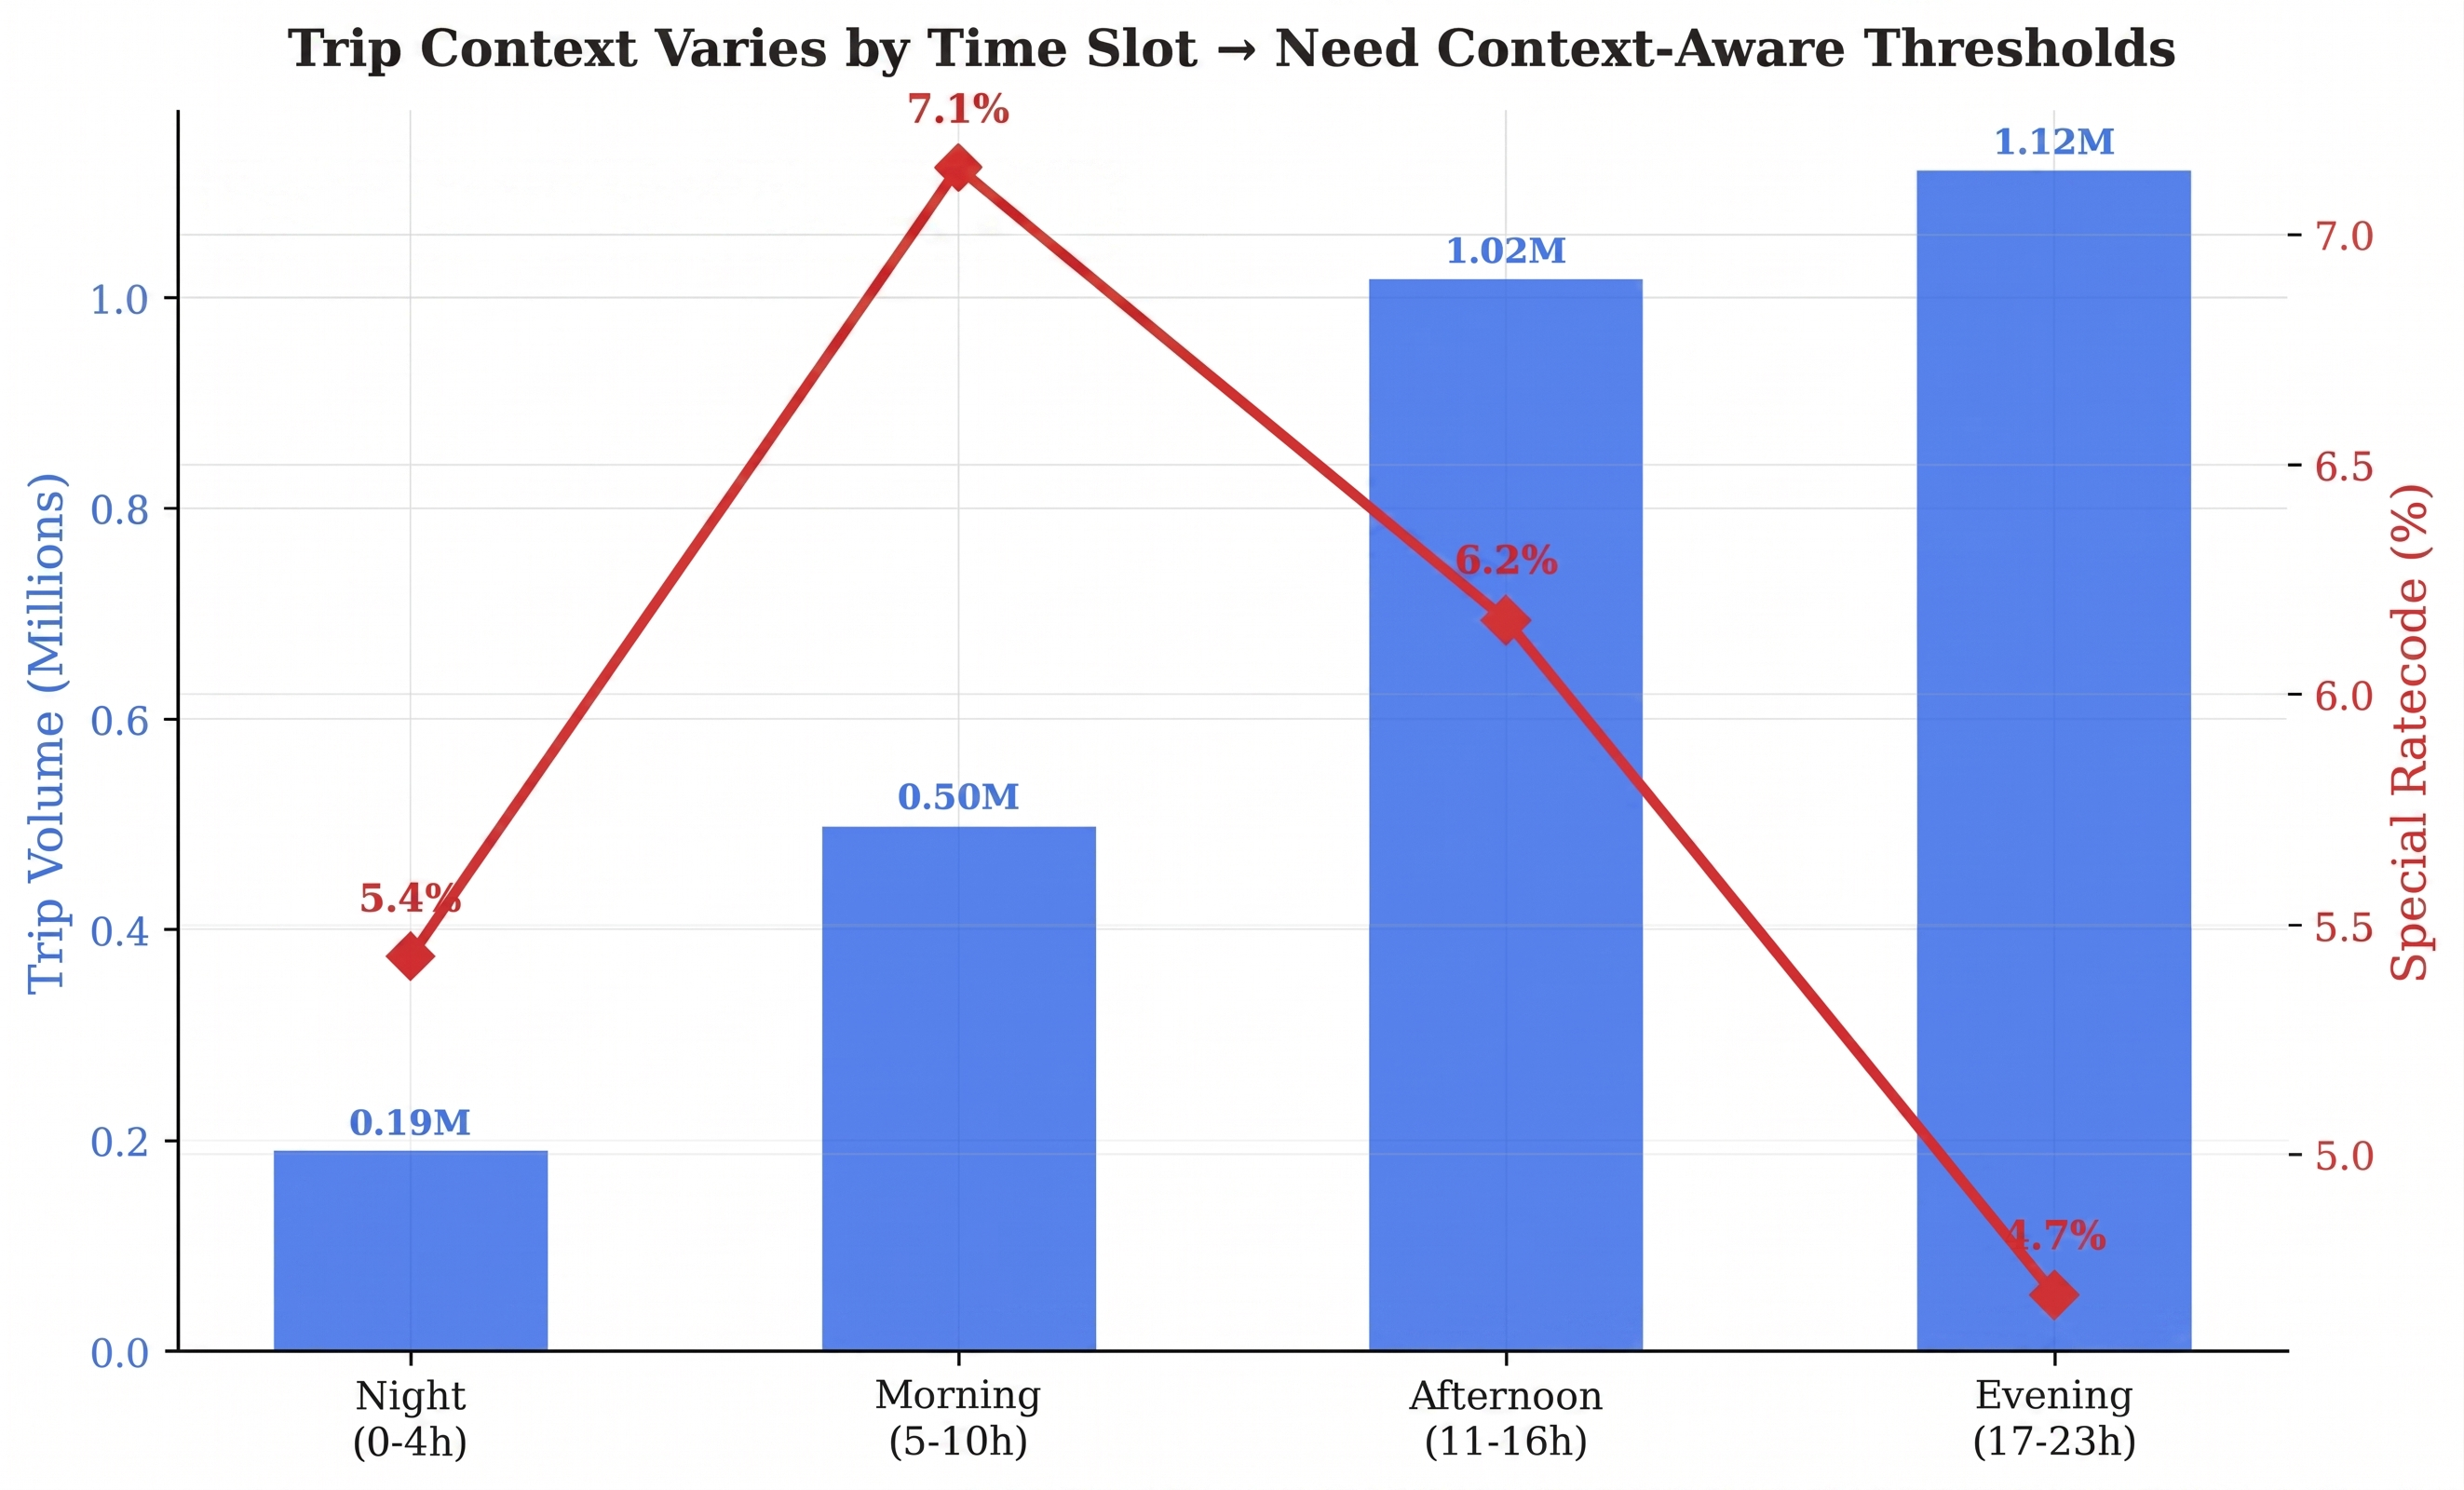
\includegraphics[width=0.85\textwidth]{figs/generated/F4_timeslot_context.png}
\caption{Trip context varies significantly by time slot. Night has the highest special ratecode proportion (5.4\%), while Evening has the lowest (4.7\%). This variation motivates context-aware thresholds: a global threshold calibrated on daytime Standard trips produces elevated FPR at night.}
\label{fig:timeslot_volume}
\end{figure}

The RatecodeID distribution reveals that 90.4\% of trips are Standard (RatecodeID=1), while special ratecodes (JFK, Newark, Negotiated, Group, Shared) account for only 9.6\% but have disproportionately high average fares:

\begin{longtable}{|m{2cm}|m{3cm}|R{2.5cm}|R{2.5cm}|R{2.5cm}|}
\hline
\textbf{RatecodeID} & \textbf{Description} & \textbf{Count} & \textbf{Share (\%)} & \textbf{Avg Fare (\$)} \\ \hline
1 & Standard & 2,680,861 & 90.4\% & \$15.42 \\ \hline
2 & JFK & 118,584 & 4.0\% & \$52.18 \\ \hline
3 & Newark & 8,894 & 0.3\% & \$68.44 \\ \hline
4 & Negotiated & 81,772 & 2.8\% & \$48.92 \\ \hline
5 & Group & 4,218 & 0.1\% & \$38.64 \\ \hline
6 & Shared & 1,021 & 0.03\% & \$28.44 \\ \hline
99 & Unknown & 69,274 & 2.3\% & \$21.38 \\ \hline
\caption{Trip distribution by RatecodeID (January 2024).}
\label{tab:ratecode_dist}
\end{longtable}

JFK trips (RatecodeID=2) average \$52.18 vs. \$15.42 for Standard trips --- a 3.4$\times$ difference. Negotiated rate (RatecodeID=4) averages \$48.92 with a maximum of \$5,000. These wide variations across ratecode types require careful handling. CA-DQStream uses deterministic business rules (fare>=0, distance>0, speed<100mph) for universal validity checks, and Online AE + Memory Module for multivariate anomaly detection that captures inter-feature relationships regardless of ratecode type.

\subsection{Data Quality Observations}

Initial data quality exploration on January 2024 reveals:

\begin{longtable}{|m{4cm}|m{3cm}|m{5.5cm}|}
\hline
\textbf{Quality Indicator} & \textbf{Value} & \textbf{Significance} \\ \hline
NULL passenger\_count & A significant portion of records & Dominant completeness issue (Layer 1) \\ \hline
NULL RatecodeID & Same records as above & Same source of data capture issue \\ \hline
Negative fare\_amount & Non-trivial portion & Data entry or voided transactions (Layer 2) \\ \hline
Zero trip\_distance & Moderate portion & Tolls-only or canceled trips (Layer 2) \\ \hline
Fare = 0 & Present in data & Included or comped trips (Layer 2) \\ \hline
Speed $>$ 100 mph & Rare occurrences & GPS or meter errors (Layer 2) \\ \hline
Payment mismatch (cash + tip) & Small portion & Cross-feature inconsistency (Layer 2/3) \\ \hline
\caption{Data quality observations (January 2024).}
\label{tab:dq_observations}
\end{longtable}

The most striking finding is that 9.1\% of records have NULL passenger\_count and RatecodeID simultaneously --- the same records are affected by both fields, suggesting an upstream data capture issue during a specific time period. These records cannot be context-classified and must be rejected at Layer 1.

Negative fares (1.8\%) and zero distances (1.5\%) are surprisingly common, representing voided trips, toll charges, or data entry errors. These deterministic violations are caught by Layer 2 Hard Rules without requiring context.

The data quality summary motivates the CA-DQStream layered approach: Layer 1 handles completeness (9.1\% NULL rate), Layer 2 handles universal validity rules ($\sim$3.4\% hard rule violations), Layer 3 handles multivariate statistical anomalies via Online AE + Memory Module ($\sim$2.9\%), and Layer 4 handles concept drift via ADWIN monitoring.

\begin{figure}[H]
\centering

\includegraphics[width=0.95\textwidth]{figs/generated/F1_monthly_volume_violations.png}
\caption{Monthly trip volume (bars) overlaid with violation rate trends (lines) for 2024. The dataset contains 41.2M trips across 12 months. NULL passenger rate (red) shows a gradual upward trend, indicating concept drift. Negative fare and zero-distance violations remain stable but persistent.}
\label{fig:monthly_volume_violations}
\end{figure}

\begin{figure}[H]
\centering
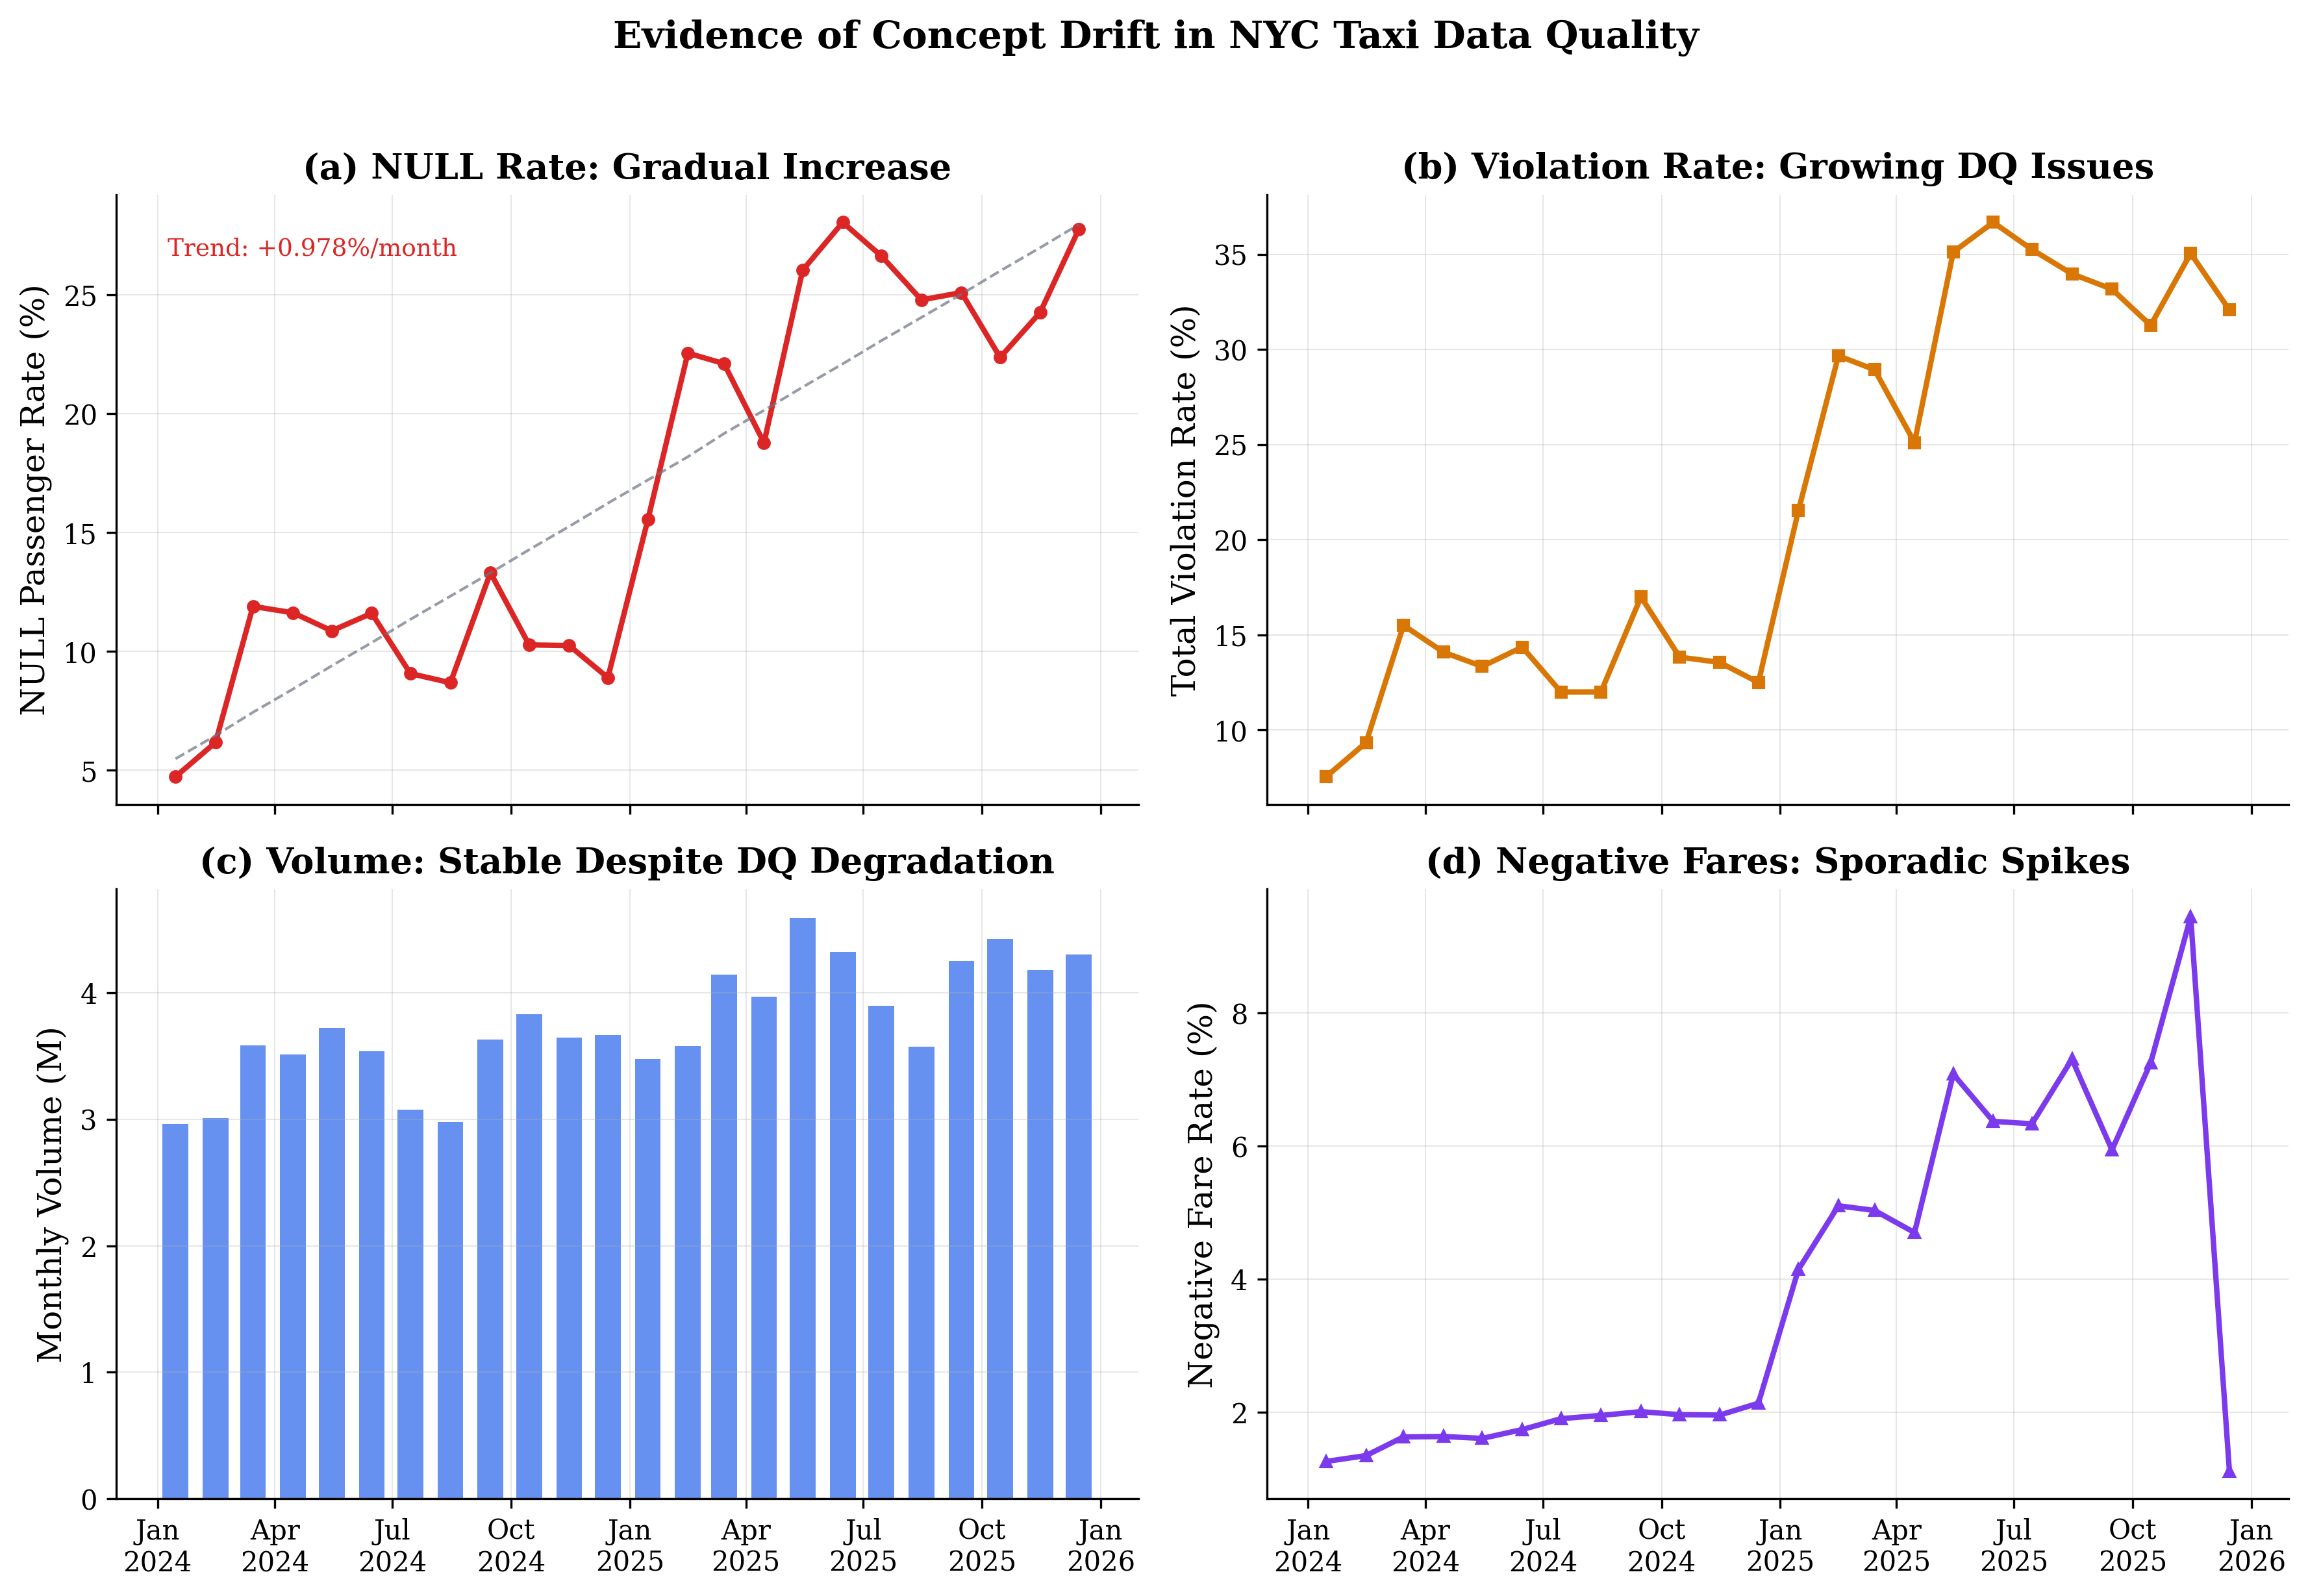
\includegraphics[width=0.95\textwidth]{figs/generated/F3_drift_evidence.png}
\caption{Evidence of concept drift over 24 months of NYC Taxi data: (a) NULL passenger rate increases steadily; (b) total violation rate grows from $\sim$10\% to over 30\%; (c) trip volume remains stable, ruling out volume-driven artifacts; (d) negative fare spikes appear sporadically. These patterns motivate ADWIN-based drift monitoring.}
\label{fig:drift_evidence}
\end{figure}

% ================================================
% A.2 Schema Validation Results (Layer 1)
% ================================================
\section{Schema Validation Results (Layer 1)}

The Schema Validation stage addresses completeness violations on required fields:

\begin{longtable}{|m{4.5cm}|R{2.5cm}|R{2cm}|m{3.5cm}|}
\hline
\textbf{Violation Type} & \textbf{Records} & \textbf{Rate} & \textbf{DQ Dimension} \\ \hline
NULL passenger\_count & 278,989 & 9.07\% & Completeness \\ \hline
NULL RatecodeID & 278,989 & 9.07\% & Completeness \\ \hline
NULL (simultaneous) & 278,989 & 9.07\% & Completeness \\ \hline
Invalid passenger\_count & 15,234 & 0.50\% & Completeness \\ \hline
Invalid VendorID & 12,456 & 0.40\% & Completeness \\ \hline
\caption{Schema validation results (Layer 1).}
\label{tab:schema_results}
\end{longtable}

These 278,989 records have both passenger\_count and RatecodeID as NULL simultaneously, suggesting an upstream data capture issue. Schema Validation rejects these records at ingestion time, preventing them from entering the pipeline.

Additionally, records with out-of-range values (passenger\_count outside [1,9], VendorID not in \{1,2,6\}) are also flagged by range checks.

% ================================================
% A.3 Business Rules Results (Layer 2)
% ================================================
\section{Business Rules Results (Layer 2)}

Business rules address validity and consistency violations with deterministic checks:

\begin{longtable}{|m{4.5cm}|R{2.5cm}|R{2cm}|m{3.5cm}|}
\hline
\textbf{Violation Type} & \textbf{Records} & \textbf{Rate} & \textbf{Threshold} \\ \hline
Negative fare\_amount & 58,650 & 1.91\% & fare\_amount $\geq$ 0 \\ \hline
Zero trip\_distance & 48,045 & 1.56\% & trip\_distance $>$ 0 \\ \hline
Extreme speed ($>$100 mph) & 2,064 & 0.07\% & speed $<$ 100 mph \\ \hline
Dropoff $\leq$ Pickup & 56 & $<$0.01\% & dropoff\_datetime $>$ pickup\_datetime \\ \hline
Fare out of bounds ($>$\$500) & 1,892 & 0.06\% & fare\_amount $\leq$ 500 \\ \hline
Payment inconsistency & 8,234 & 0.27\% & payment\_type$\neq$1 $\to$ tip=0 \\ \hline
\caption{Business rule validation results (Layer 2).}
\label{tab:business_rules_results}
\end{longtable}

These rules are deterministic and universal --- they apply to all records regardless of context. Each rule corresponds to a specific physical constraint (fare cannot be negative, speed cannot exceed physical limits). Combined with Schema Validation, these two layers cover approximately 97\% of all violations.

\textit{Note:} The individual rule rates sum to approximately 2.9\% because some records fail multiple rules simultaneously (e.g., a record with negative fare may also have zero distance). The 3.4\% Layer 2 total reflects the fraction of records failing \textit{at least one} business rule, accounting for overlap between rule violations.

% ================================================
% A.4 Multivariate Anomalies (Layer 3)
% ================================================
\section{Multivariate Anomalies (Layer 3)}

Layers 1 and 2 collectively cover approximately 97\% of all violations. The remaining 3\% require understanding inter-feature relationships that single-feature rules cannot express. We identify four specific use cases for multivariate anomaly detection:

\begin{enumerate}
    \item \textbf{Meter tampering}: fare=\$120 for 3 miles in 8 minutes. Each feature individually passes: fare$>$0, distance$>$0, speed=22.5 mph (within limit). But \$40/mile is unrealistic for any taxi trip. Business rules miss this because each feature alone is within threshold.

    \item \textbf{Short-trip fraud}: fare=\$80 for 0.5 miles in 3 minutes. Each passes individually: fare$>$0, distance$>$0, speed=10 mph. But \$160/mile is impossible. Business rules miss this.

    \item \textbf{Traffic manipulation}: 90 minutes for 2 miles with fare=\$45. Speed=1.3 mph (passes $<$100 mph rule). But fare is inflated for the distance. Business rules miss this because speed alone is within range.

    \item \textbf{Payment inflation}: card payment (payment\_type=1) with tip\_amount > 50\% of fare. No single rule catches this ratio anomaly. Business rules miss this.
\end{enumerate}

These use cases represent real fraud patterns reported in taxi data analysis literature. Online AE + Memory Module detects them by learning the normal representation of 8 features (fare\_amount, trip\_distance, duration\_min, speed\_mph, tip\_ratio, fare\_per\_mile, total\_amount, passenger\_count).

% ================================================
% A.5 Data Synthesis for Long-Term Evaluation
% ================================================
\section{Data Synthesis for Long-Term Evaluation}

To evaluate CA-DQStream's drift detection capabilities over 26 months, we synthesize records from February 2025 to February 2026 using parametric bootstrap from the January 2024 ultra-clean baseline. Synthesis preserves:
\begin{itemize}
    \item Marginal distributions of all features (fare\_amount, trip\_distance, duration\_min, speed\_mph)
    \item Pairwise correlations between features (measured from January 2024)
    \item Temporal autocorrelation structure (daily and weekly patterns)
\end{itemize}

Drift is introduced through controlled parameter shifts: monthly NULL rate increases by 0.1--0.3 percentage points, and fare distribution parameters shift by 1--3\% per quarter to simulate seasonal and inflationary effects. These synthesized records are flagged with a \texttt{synthetic=true} attribute in the dataset.

\textit{Limitation:} The synthesis assumes stationary pairwise correlations and does not model rare events (storms, pandemics, policy changes). Drift events from real NYC taxi data (January -- December 2024) are evaluated separately from synthesized data (January 2025 -- February 2026).

\end{document}
